% SCRUM-103 / A2-T2.1 — Fragment cho báo cáo Assignment 2.
% Canonical content: docs/diagrams/A2_T2.1_Activity_Diagram_Checkout.md
% Source diagrams:
%   - docs/diagrams/activity-checkout.puml (Tổng thể End-to-End)
%   - docs/diagrams/activity-checkout-phase1-order.puml (Pha 1: Tạo Order & Khởi tạo thanh toán)
%   - docs/diagrams/activity-checkout-phase2-payment.puml (Pha 2A: Tương tác VNPay, Return URL độc lập & Kết quả Customer)
%   - docs/diagrams/activity-checkout-phase3-reconciliation.puml (Pha 2B: Xử lý IPN, Chu kỳ Scheduler Đối soát & TTL/Grace)
% Rendered exports:
%   - docs/diagrams/activity-checkout*.svg / .pdf
%   - docs/report/assets/activity-checkout*.pdf
% Yêu cầu gói trong preamble chính: \usepackage{graphicx}, \usepackage{longtable}, \usepackage{array}

\section{Activity Diagram --- Luồng Checkout (\texttt{UC-A2-CHECKOUT-001})}
\label{sec:a2-activity-checkout}

\noindent\textbf{Task:} SCRUM-103 / A2-T2.1\par
\noindent\textbf{Trạng thái:} DRAFT -- đã cập nhật phản hồi Review lần 2 của PR \#4 (\texttt{R-01}..\texttt{R-06} \& tối ưu bố cục trình bày)\par
\noindent\textbf{Ngày soạn:} 08/11/2026\par
\noindent\textbf{Baseline đối chiếu:} \texttt{A1-final} (\texttt{1951dc124c83359556f04adb6ba3f0ee9f22fce4})\par
\noindent\textbf{Tệp nguồn \& kết xuất:} \texttt{docs/diagrams/activity-checkout.puml}, \texttt{docs/diagrams/activity-checkout-phase1-order.puml}, \texttt{docs/diagrams/activity-checkout-phase2-payment.puml}, \texttt{docs/diagrams/activity-checkout-phase3-reconciliation.puml} (cùng các bản xuất \texttt{.svg} và \texttt{.pdf} đồng bộ)\par

\subsection{Mục tiêu và nguyên tắc kế thừa từ Assignment 1}

Sơ đồ hoạt động (Activity Diagram) của Task~2.1 mô hình hóa luồng nghiệp vụ end-to-end cho Use Case trọng tâm \texttt{UC-A2-CHECKOUT-001} (\emph{Đặt hàng và thanh toán}), kế thừa bốn sơ đồ con trong bộ tạo phẩm Assignment~1 (\texttt{docs/diagram/Activity-Final.drawio.svg}: \texttt{AD-02} Quy trình đặt món tổng quan, \texttt{AD-03} Tạo đơn hàng, \texttt{AD-04} Thanh toán và \texttt{AD-06} Hủy đơn hàng quá 15 phút) và chuẩn hóa theo Requirements Specification v3.1 cùng API Contract v4.0.
\par

So với phiên bản A1 vốn chỉ chia hai phân vùng tổng quát (\emph{Người dùng} và \emph{Hệ thống}) và chỉ mô tả thanh toán giả lập (\texttt{CARD}/\texttt{WALLET}), sơ đồ chuẩn hóa ở Assignment~2 giải quyết trọn vẹn các yêu cầu của mục Task~2.1:
\begin{itemize}
  \item Tách rõ \textbf{5 swimlane} theo đúng kiến trúc thực tế: \texttt{Customer}, \texttt{Next.js Frontend}, \texttt{NestJS Backend}, \texttt{PostgreSQL DB} và actor ngoài \texttt{VNPay Sandbox}.
  \item Chuẩn hóa toàn bộ các \textbf{Decision Node (D1--D22)} theo quy tắc thống nhất (\texttt{R-02}): nhánh \texttt{then} luôn mang nhãn khẳng định \texttt{Có (...)} khớp trực tiếp với câu hỏi nghi vấn trong hình thoi, và nhánh \texttt{else} luôn mang nhãn phủ định \texttt{Không (...)}.
  \item Biểu diễn \textbf{Luồng 1 (Browser Redirect qua Return URL)} và \textbf{Luồng 2 (Server-to-Server IPN / Scheduler đối soát nội bộ)} là hai luồng hoàn toàn độc lập (\texttt{R-03}), sử dụng \texttt{fork ... end merge} và kết thúc độc lập ở luồng nền (\texttt{stop}), loại bỏ điểm đồng bộ giả (Join Bar) để phản ánh đúng thực tế Backend vẫn hoàn tất đơn ngay cả khi \texttt{Customer} đóng trình duyệt.
  \item Mô hình hóa rõ \textbf{vòng lặp chu kỳ Scheduler đánh giá lại theo thời gian (\texttt{R-04})}: khi giao dịch còn \texttt{PENDING} trước mốc \(E = \text{createdAt} + 15\text{m}\) hoặc vừa bước vào cửa sổ Grace \(5\text{ phút}\) \([E, G)\) với \(G = E + 5\text{m}\) (\texttt{RECONCILING}), hệ thống lưu trạng thái vào Database và đi qua bước chờ sự kiện tiếp theo (IPN đến muộn hoặc chu kỳ kích hoạt kế tiếp của \texttt{PaymentReconciliationScheduler} / \texttt{OrderExpirationService}) trước khi đánh giá lại các mốc \(E\) và \(G\).
  \item Đảm bảo tất cả các nhánh thanh toán --- bao gồm \textbf{VNPay Sandbox (\texttt{Main Flow})}, \textbf{đơn hàng \(0\,\text{đ}\) (\texttt{AF-03: ZERO\_AMOUNT})} và \textbf{chế độ Mock test/demo (\texttt{AF-04})} --- đều đi qua bước lưu bền vững tại \texttt{PostgreSQL DB}, đồng bộ về \texttt{Next.js Frontend} để hiển thị giao diện và kết thúc tại \texttt{Customer} (\texttt{R-05}).
  \item Chia sơ đồ thành \textbf{3 hình tách pha rõ nét} (\texttt{Pha 1}, \texttt{Pha 2A}, \texttt{Pha 2B}) bên cạnh bản tổng thể end-to-end để tối ưu tỉ lệ hiển thị trên trang báo cáo A4 (\texttt{R-06}).
\end{itemize}

\subsection{Phân vùng trách nhiệm (Swimlanes) và các nút quyết định chính}

\begingroup\small
\renewcommand{\arraystretch}{1.2}
\begin{longtable}{>{\raggedright\arraybackslash}p{0.20\linewidth}>{\raggedright\arraybackslash}p{0.44\linewidth}>{\raggedright\arraybackslash}p{0.28\linewidth}}
\hline
\textbf{Swimlane} & \textbf{Hành động chính trên sơ đồ} & \textbf{Ràng buộc / Bất biến} \\ \hline
\endfirsthead
\hline
\textbf{Swimlane} & \textbf{Hành động chính trên sơ đồ} & \textbf{Ràng buộc / Bất biến} \\ \hline
\endhead
\texttt{Customer} & Mở giỏ hàng, nhập mã coupon (tùy chọn), nhấn Đặt hàng; xác nhận thanh toán hoặc chọn Retry; thao tác trên cổng VNPay Sandbox; nhận kết quả cuối cùng cho cả 3 nhánh (\texttt{VNPay}, \texttt{ZERO\_AMOUNT}, \texttt{Mock}). & Chỉ được Retry khi \texttt{Order == PAYMENT\_FAILED}, còn hạn \(\text{now} < E\) và không có cờ đối soát/ngoại lệ tài chính. \\ \hline
\texttt{Next.js Frontend} & Kiểm tra JWT client-side; gửi \texttt{POST /orders}; giữ giỏ hàng cho đến khi \texttt{Order == PAID}; sinh \texttt{Idempotency-Key} (8..64 ký tự); redirect sang VNPay; nhận Return URL độc lập và gọi \texttt{GET /orders/me} (bounded polling); hiển thị kết quả cuối cùng cho \texttt{Customer}. & Không tự coi Return URL là \texttt{PAID} (\texttt{EF-11}); không tự xóa giỏ khi giao dịch còn \texttt{PENDING}. \\ \hline
\texttt{NestJS Backend} & Thực thi \texttt{JwtAuthGuard}, \texttt{ValidationPipe}, \texttt{MockPaymentGuard}; tính giá authoritative (\texttt{round-half-up}); kiểm tra 1 Order active, \texttt{Idempotency-Key} và TTL; khởi tạo VNPay; xử lý độc lập ở nền qua IPN (\texttt{GET /payments/vnpay/ipn}) hoặc chu kỳ Scheduler đối soát nội bộ; thực thi \texttt{Shared Finalization}. & Không tin cậy giá/discount từ client; khóa bản ghi theo thứ tự chuẩn để chống race condition (\texttt{EF-13 / BR-C05}). \\ \hline
\texttt{PostgreSQL DB} & Kiểm tra Order active, tồn kho và coupon trong transaction; lưu snapshot \texttt{Order}/\texttt{OrderItem}; trừ/hoàn stock; chuyển trạng thái coupon (\texttt{HELD} \(\rightarrow\) \texttt{CONSUMED} hoặc release); cập nhật \texttt{Payment} và điểm tích lũy nguyên tử. & Rollback toàn bộ khi lỗi (\texttt{EF-15}); mỗi tài nguyên chỉ được trừ/tiêu thụ hoặc hoàn trả đúng một lần. \\ \hline
\texttt{VNPay Sandbox} & Hiển thị cổng thanh toán cho nhánh \texttt{totalVnd > 0}; kích hoạt 2 luồng độc lập: (1) Browser Redirect qua Return URL về Frontend và (2) Server-to-Server IPN về Backend. & Chỉ tham gia trên nhánh VNPay; không tham gia nhánh \texttt{ZERO\_AMOUNT} hoặc Mock. \\ \hline
\end{longtable}
\endgroup

\subsection{Tóm tắt luồng hoạt động theo 3 sơ đồ tách pha}

\begin{enumerate}
  \item \textbf{Pha 1 --- Tạo Order \texttt{PENDING}, giữ tài nguyên và khởi tạo thanh toán (Hình~\ref{fig:a2-activity-checkout-phase1}):}
  \begin{itemize}
    \item \emph{Kiểm tra đăng nhập và tạo đơn (\texttt{POST /orders}):} \texttt{Next.js Frontend} kiểm tra phiên JWT (\textbf{D1}: \texttt{Đã đăng nhập?} \(\rightarrow\) \texttt{Có} gửi \texttt{POST /orders} / \texttt{Không [EF-01]} yêu cầu đăng nhập, giữ giỏ). Tại \texttt{NestJS Backend}, \textbf{D2} (\texttt{JWT \& DTO hợp lệ?}) trả \texttt{401/400} nếu \texttt{Không}. Trong DB Transaction nguyên tử, hệ thống xét \textbf{D3} (\texttt{Đã có Order active?} \(\rightarrow\) nếu \texttt{Có} trả \texttt{409 PENDING\_ORDER\_EXISTS} --- \texttt{EF-05 / BR-C02}) và \textbf{D4} (\texttt{Đủ stock \& Coupon hợp lệ?} \(\rightarrow\) nếu \texttt{Không} thì rollback nguyên tử và trả \texttt{409 INSUFFICIENT\_STOCK} hoặc \texttt{400/409} lỗi coupon --- \texttt{EF-04 / EF-15}). Nếu \texttt{Có}, hệ thống tính giá authoritative phía server (\texttt{BR-C01}), đặt \(\text{expiresAt} = E = \text{createdAt} + 15\text{m}\), tạo \texttt{Order (PENDING)}, trừ tồn kho và giữ coupon (\texttt{HELD}).
    \item \emph{Phân nhánh khởi tạo thanh toán:} Sau khi kiểm tra quyền sở hữu (\texttt{EF-02}), \texttt{Idempotency-Key} (\texttt{AF-10 / EF-06}), hạn TTL (\texttt{EF-08}) và cờ chặn (\texttt{EF-07}) tại \textbf{D5} (\texttt{Đủ điều kiện thanh toán?}), luồng rẽ qua:
    \begin{itemize}
      \item \textbf{D6 (\texttt{Đơn hàng 0đ (totalVnd == 0)?}):} Nếu \texttt{Có [AF-03, BR-C07]}, xử lý \texttt{POST /payments/zero-amount}, commit nguyên tử \texttt{Payment = SUCCESS (0đ)}, \texttt{Order = PAID}, \texttt{Coupon HELD \(\rightarrow\) CONSUMED}, \texttt{loyaltyPointsEarned = 0} rồi chuyển sang Pha~2A để hiển thị cho \texttt{Customer}.
      \item \textbf{D7--D9 (\texttt{Dùng chế độ Mock [AF-04]?}):} Nếu \texttt{Có}, xét \textbf{D8} (\texttt{Cho phép chạy Mock?}: nếu \texttt{Không [BR-C09]} trả \texttt{403 MOCK\_PAYMENT\_DISABLED}). Tại \textbf{D9} (\texttt{Thẻ 0002 / Ví 0000 từ chối?}), nếu \texttt{Có} thì commit \texttt{Payment = FAILED}, \texttt{Order = PAYMENT\_FAILED}; nếu \texttt{Không} thì commit \texttt{Payment = SUCCESS}, \texttt{Order = PAID}, rồi chuyển sang Pha~2A.
      \item \textbf{Luồng chính VNPay Sandbox (\texttt{D6 = Không} \& \texttt{D7 = Không}):} Xử lý \texttt{POST /payments/vnpay/initiate}, tạo bản ghi \texttt{Payment (PENDING)} với \texttt{vnp\_TxnRef} duy nhất và trả \texttt{paymentUrl} ký \texttt{HMAC-SHA512}.
    \end{itemize}
  \end{itemize}

  \item \textbf{Pha 2A --- Tương tác VNPay, Return URL độc lập với IPN và Hiển thị kết quả cho Customer (Hình~\ref{fig:a2-activity-checkout-phase2a}):}
  \begin{itemize}
    \item Tại \textbf{D10} (\texttt{Hoàn tất đồng bộ ở Pha 1?}), nếu \texttt{Có [ZERO\_AMOUNT / Mock]}, \texttt{Next.js Frontend} nhận trực tiếp kết quả \texttt{PAID}/\texttt{PAYMENT\_FAILED} và hiển thị cho \texttt{Customer}.
    \item Nếu \texttt{Không [VNPay PENDING]}, trình duyệt redirect sang \texttt{VNPay Sandbox}. Sau khi \texttt{Customer} thao tác, hai luồng độc lập được kích hoạt mà \textbf{không có Join Bar đồng bộ giả}:
    \begin{itemize}
      \item \emph{Luồng 1 (Browser Redirect --- độc lập với IPN):} Xét \textbf{D11} (\texttt{Trình duyệt quay về Return URL?}): nếu \texttt{Có}, Frontend nhận Return URL (\texttt{EF-11}: không tự coi là \texttt{PAID}) và gọi \texttt{GET /orders/me}; nếu \texttt{Không: Đóng trình duyệt}, xét \textbf{D12} (\texttt{Khách mở lại trang Đơn hàng?}): nếu \texttt{Không} thì phiên trình duyệt kết thúc ngay (\texttt{stop}), còn nếu \texttt{Có} thì gọi \texttt{GET /orders/me} đọc kết quả từ DB.
      \item \emph{Luồng 2 (Server-to-Server IPN / Scheduler --- độc lập với trình duyệt):} Backend thực thi xử lý IPN và chu kỳ đối soát ở nền (chi tiết tại Pha~2B), lưu bền vững vào \texttt{PostgreSQL DB} và kết thúc độc lập (\texttt{stop}).
    \end{itemize}
  \end{itemize}

  \item \textbf{Pha 2B --- Xử lý IPN, Chu kỳ Scheduler Đối soát \texttt{QueryDR} và Hết hạn TTL \(15\text{m}\) / Grace \(5\text{m}\) (Hình~\ref{fig:a2-activity-checkout-phase2b}):}
  \begin{itemize}
    \item Tại \textbf{D13} (\texttt{Nhận được webhook IPN từ VNPay?}), nếu \texttt{Có}, Backend kiểm tra chữ ký \texttt{HMAC-SHA512}, \texttt{TmnCode}, \texttt{vnp\_TxnRef} và số tiền snapshot tại \textbf{D14} (\texttt{Chữ ký \& số tiền hợp lệ?}: nếu \texttt{Không [EF-10]} thì từ chối Finalization và dừng); nếu \texttt{Không: Mất IPN / Timeout}, Scheduler định kỳ kích hoạt đối soát nội bộ (\texttt{VnpayQuerydrService / OrderExpirationService}).
    \item Hệ thống đi vào vòng lặp đánh giá theo chu kỳ (\texttt{repeat ... repeat while (Vẫn đang PENDING / RECONCILING?)}), khóa bản ghi theo thứ tự chuẩn (\texttt{BR-C05}) và xét chuỗi Decision Node:
    \begin{itemize}
      \item \textbf{D15 (\texttt{Kết quả giao dịch là SUCCESS [00]?}) = Có \(\rightarrow\) D16 (\texttt{Đúng hạn paidAt <= E \& chưa hủy?}):} Nếu \texttt{Có [Main Flow]} thì xác định \texttt{Payment = SUCCESS}, \texttt{Order = PAID} (\texttt{break}); nếu \texttt{Không: Thanh toán trễ [EF-12]} thì ghi nhận ngoại lệ tài chính \texttt{hasFinancialException = true}, \texttt{REQUIRES\_REVIEW}, không hồi sinh đơn (\texttt{break}).
      \item \textbf{D17 (\texttt{Kết quả là Terminal FAILED?}) = Có [AF-05] \(\rightarrow\) D18 (\texttt{Còn hạn TTL 15 phút (now < E)?}):} Nếu \texttt{Có} thì \texttt{Payment = FAILED}, \texttt{Order = PAYMENT\_FAILED} (giữ stock/coupon để Retry, \texttt{break}); nếu \texttt{Không} (\(\text{now} \ge E\)) thì \texttt{Payment = FAILED}, \texttt{Order = CANCELLED} (\texttt{break}).
      \item \textbf{D17 = Không (\texttt{UNKNOWN}) \(\rightarrow\) D19 (\texttt{Đã tới mốc TTL 15 phút (now >= E)?}):} Nếu \texttt{Không: now < E}, giữ \texttt{Order = PENDING, Payment = PENDING} trong DB rồi chuyển xuống bước \textbf{chờ chu kỳ Scheduler kế tiếp hoặc sự kiện IPN đến muộn}. Nếu \texttt{Có: now >= E}, xét \textbf{D20} (\texttt{Có VNPay PENDING tạo trước E?}): nếu \texttt{Không [AF-08]} thì hủy đơn ngay tại mốc \(E\) (\texttt{break}); nếu \texttt{Có: Xét Grace [AF-07]} thì xét \textbf{D21} (\texttt{Đã quá mốc Grace 5 phút (now >= G)?}):
      \begin{itemize}
        \item Khi \(E \le \text{now} < G\) (\textbf{D21 = Không}): Lưu trạng thái trong cửa sổ Grace \([E, G)\) (\texttt{Order = PENDING, reconciliationState = RECONCILING}, chặn tạo attempt/Order mới \texttt{BR-C03}), sau đó \textbf{chờ chu kỳ Scheduler kế tiếp hoặc sự kiện IPN đến muộn} (\textbf{D22 = Có: Tới chu kỳ kế tiếp}) để đánh giá lại khi thời gian tiến tới mốc \(G\).
        \item Khi \(\text{now} \ge G\) (\textbf{D21 = Có [AF-09, BR-C10]}): Xác định hết hạn sau cửa sổ Grace tại mốc \(G\) (\texttt{Order \(\rightarrow\) CANCELLED}, hoàn trả stock \& giải phóng coupon 1 lần; giữ \texttt{Payment.status = PENDING} kèm \texttt{reconciliationState = REQUIRES\_REVIEW}, \texttt{break}).
      \end{itemize}
    \end{itemize}
    \item Khi đã có kết cục cuối (\textbf{D22 = Không: Đã có kết cục}), hệ thống commit nguyên tử vào \texttt{PostgreSQL DB} và kết thúc (\texttt{stop}).
  \end{itemize}
\end{enumerate}

\subsection{Ghi chú đối chiếu với Implementation \texttt{A1-final}}

\begin{itemize}
  \item \textbf{Endpoint tra cứu trạng thái phía Frontend:} Trong mã nguồn \texttt{A1-final}, trang xác nhận đơn hàng đồng bộ dữ liệu thực tế qua \texttt{GET /orders/me} (đã triển khai đầy đủ ở cả Frontend và Backend). Endpoint \texttt{GET /payments/:paymentId/status} thuộc đặc tả API Contract v4.0 (\texttt{API-03}) chưa có route controller tương ứng ở backend tại \texttt{A1-final}, nên được chú thích rõ là \texttt{[VERIFY]} trên sơ đồ.
  \item \textbf{Đối soát QueryDR:} Các thành phần \texttt{VnpayIpnController}, \texttt{PaymentFinalizationService}, \texttt{OrderExpirationService}, \texttt{VnpayQuerydrService} và \texttt{PaymentReconciliationScheduler} đã hiện diện trong mã nguồn và unit/integration test; kiểm thử E2E trực tiếp với máy chủ QueryDR của VNPay Sandbox thực tế thuộc phạm vi hoãn theo \texttt{ADR-P2-QueryDR-Sandbox-E2E-Deferred}.
\end{itemize}

\subsection{Sơ đồ Activity Diagram Checkout (Tách Pha \& Tổng thể)}

\begin{figure}[htbp]
\centering
\IfFileExists{docs/report/assets/activity-checkout-phase1-order.pdf}{%
  \includegraphics[width=\linewidth,height=0.84\textheight,keepaspectratio]{docs/report/assets/activity-checkout-phase1-order.pdf}%
}{%
  \IfFileExists{../assets/activity-checkout-phase1-order.pdf}{%
    \includegraphics[width=\linewidth,height=0.84\textheight,keepaspectratio]{../assets/activity-checkout-phase1-order.pdf}%
  }{%
    \IfFileExists{docs/diagrams/activity-checkout-phase1-order.pdf}{%
      \includegraphics[width=\linewidth,height=0.84\textheight,keepaspectratio]{docs/diagrams/activity-checkout-phase1-order.pdf}%
    }{%
      \fbox{\parbox{0.85\linewidth}{\centering
      Sơ đồ Pha 1 nằm tại \texttt{docs/diagrams/activity-checkout-phase1-order.pdf} và \texttt{docs/report/assets/activity-checkout-phase1-order.pdf}.}}%
    }%
  }%
}
\caption{Activity Diagram Checkout --- \textbf{Pha 1}: Kiểm tra phiên JWT, tạo Order \texttt{PENDING} nguyên tử và phân nhánh khởi tạo thanh toán (\texttt{ZERO\_AMOUNT}, \texttt{Mock}, \texttt{VNPay Sandbox}).}
\label{fig:a2-activity-checkout-phase1}
\end{figure}

\begin{figure}[htbp]
\centering
\IfFileExists{docs/report/assets/activity-checkout-phase2-payment.pdf}{%
  \includegraphics[width=\linewidth,height=0.84\textheight,keepaspectratio]{docs/report/assets/activity-checkout-phase2-payment.pdf}%
}{%
  \IfFileExists{../assets/activity-checkout-phase2-payment.pdf}{%
    \includegraphics[width=\linewidth,height=0.84\textheight,keepaspectratio]{../assets/activity-checkout-phase2-payment.pdf}%
  }{%
    \IfFileExists{docs/diagrams/activity-checkout-phase2-payment.pdf}{%
      \includegraphics[width=\linewidth,height=0.84\textheight,keepaspectratio]{docs/diagrams/activity-checkout-phase2-payment.pdf}%
    }{%
      \fbox{\parbox{0.85\linewidth}{\centering
      Sơ đồ Pha 2A nằm tại \texttt{docs/diagrams/activity-checkout-phase2-payment.pdf} và \texttt{docs/report/assets/activity-checkout-phase2-payment.pdf}.}}%
    }%
  }%
}
\caption{Activity Diagram Checkout --- \textbf{Pha 2A}: Tương tác \texttt{VNPay Sandbox}, phân tách độc lập luồng trình duyệt Return URL và luồng nền IPN/Scheduler (không đồng bộ giả) và hiển thị kết quả cuối cùng cho \texttt{Customer}.}
\label{fig:a2-activity-checkout-phase2a}
\end{figure}

\begin{figure}[htbp]
\centering
\IfFileExists{docs/report/assets/activity-checkout-phase3-reconciliation.pdf}{%
  \includegraphics[width=\linewidth,height=0.84\textheight,keepaspectratio]{docs/report/assets/activity-checkout-phase3-reconciliation.pdf}%
}{%
  \IfFileExists{../assets/activity-checkout-phase3-reconciliation.pdf}{%
    \includegraphics[width=\linewidth,height=0.84\textheight,keepaspectratio]{../assets/activity-checkout-phase3-reconciliation.pdf}%
  }{%
    \IfFileExists{docs/diagrams/activity-checkout-phase3-reconciliation.pdf}{%
      \includegraphics[width=\linewidth,height=0.84\textheight,keepaspectratio]{docs/diagrams/activity-checkout-phase3-reconciliation.pdf}%
    }{%
      \fbox{\parbox{0.85\linewidth}{\centering
      Sơ đồ Pha 2B nằm tại \texttt{docs/diagrams/activity-checkout-phase3-reconciliation.pdf} và \texttt{docs/report/assets/activity-checkout-phase3-reconciliation.pdf}.}}%
    }%
  }%
}
\caption{Activity Diagram Checkout --- \textbf{Pha 2B}: Xử lý webhook IPN, \texttt{Shared Finalization} và vòng lặp chu kỳ Scheduler đánh giá lại khi thời gian tiến tới mốc TTL \(15\text{ phút}\) (\(E\)) và mốc Grace \(5\text{ phút}\) (\(G = E + 5\text{m}\)).}
\label{fig:a2-activity-checkout-phase2b}
\end{figure}

\begin{figure}[htbp]
\centering
\IfFileExists{docs/report/assets/activity-checkout.pdf}{%
  \includegraphics[width=\linewidth,height=0.84\textheight,keepaspectratio]{docs/report/assets/activity-checkout.pdf}%
}{%
  \IfFileExists{../assets/activity-checkout.pdf}{%
    \includegraphics[width=\linewidth,height=0.84\textheight,keepaspectratio]{../assets/activity-checkout.pdf}%
  }{%
    \IfFileExists{docs/diagrams/activity-checkout.pdf}{%
      \includegraphics[width=\linewidth,height=0.84\textheight,keepaspectratio]{docs/diagrams/activity-checkout.pdf}%
    }{%
      \fbox{\parbox{0.85\linewidth}{\centering
      Sơ đồ tổng thể Activity Diagram Checkout nằm tại \texttt{docs/diagrams/activity-checkout.pdf} và \texttt{docs/report/assets/activity-checkout.pdf}.}}%
    }%
  }%
}
\caption{Activity Diagram Checkout tổng thể End-to-End (\texttt{UC-A2-CHECKOUT-001}) hợp nhất toàn bộ 5 swimlane (bản vector phóng đại không vỡ nét).}
\label{fig:a2-activity-checkout-full}
\end{figure}
